\documentclass{wissdoc}
% Autor: Roland Bless 1996-2009, bless <at> kit.edu
% ----------------------------------------------------------------
% Diplomarbeit - Hauptdokument
% ----------------------------------------------------------------
%%
%% $Id: thesis.tex 65 2012-05-10 10:32:11Z bless $
%%
%
% Zum Erstellen zweiseitiger PDFs (für Buchdruck) in der Datei "wissdoc.cls" folgende Zeile abändern:
%
% \LoadClass[a4paper,12pt,oneside]{book} % diese Klasse basiert auf ``book''
% in
%\LoadClass[a4paper,12pt,titlepage]{book} % diese Klasse basiert auf ``book''
%
%
% wissdoc Optionen: draft, relaxed, pdf --> siehe wissdoc.cls
% ------------------------------------------------------------------
% Weitere packages: (Dokumentation dazu durch "latex <package>.dtx")
\usepackage[numbers,sort&compress]{natbib}
\usepackage{hyperref}
\usepackage{amsfonts}
\usepackage{csquotes}
\usepackage[english]{babel}
\usepackage{tikz}
\usetikzlibrary{arrows}
\usetikzlibrary{arrows.meta}
\usepackage{wrapfig}
\usepackage{pgfplots}
\usepackage{readarray}
\usepackage{changes}
\usepackage{amsmath}
\usepackage{mathtools}
\mathtoolsset{showonlyrefs}  
\usepackage{float}
\restylefloat{table}
\usepackage{environ}
\makeatletter
\newsavebox{\measure@tikzpicture}
\NewEnviron{scaletikzpicturetowidth}[1]{%
	\def\tikz@width{#1}%
	\def\tikzscale{1}\begin{lrbox}{\measure@tikzpicture}%
		\BODY
	\end{lrbox}%
	\pgfmathparse{#1/\wd\measure@tikzpicture}%
	\edef\tikzscale{\pgfmathresult}%
	\BODY
}
\makeatother



\tikzset{
	treenode/.style = {align=center, inner sep=0pt, text centered,
		font=\sffamily},
	arn_n/.style = {treenode, circle, white, font=\sffamily\bfseries, draw=black,
		fill=black, text width=1.5em},% arbre rouge noir, noeud noir
}

% \usepackage{varioref}
% \usepackage{verbatim}
% \usepackage{float}    %z.B. \floatstyle{ruled}\restylefloat{figure}
% \usepackage{subfigure}
% \usepackage{fancybox} % für schattierte,ovale Boxen etc.
% \usepackage{tabularx} % automatische Spaltenbreite
% \usepackage{supertab} % mehrseitige Tabellen
% \usepackage[svnon,svnfoot]{svnver} % SVN Versionsinformation 
%% ---------------- end of usepackages -------------

%\svnversion{$Id: thesis.tex 65 2012-05-10 10:32:11Z bless $} % In case that you want to include version information in the footer

%% Informationen für die PDF-Datei
\hypersetup{
 pdfauthor={Sven Fiergolla},
 pdftitle={Improvements on RLE by preprocessing}
 pdfsubject={Not set},
 pdfkeywords={Not set}
}

% Macros, nicht unbedingt notwendig
%%%%%%%%%%%%%%%%%%%%%%%%%%%%%%%%%%%%%%%%%%%%%%%%%%%%%%%%%%
% macros.tex -- einige mehr oder weniger nuetzliche Makros
% Autor: Roland Bless 1998
%%%%%%%%%%%%%%%%%%%%%%%%%%%%%%%%%%%%%%%%%%%%%%%%%%%%%%%%%%
% $Id: macros.tex 33 2007-01-23 09:00:59Z bless $
%%%%%%%%%%%%%%%%%%%%%%%%%%%%%%%%%%%%%%%%%%%%%%%%%%%%%%%%%%


%%%%%%%%%%%%%%%%%%%%%%%
% Kommentare 
%%%%%%%%%%%%%%%%%%%%%%%
\ifnotdraftelse{
\newcommand{\Kommentar}[1]{}
}{\newcommand{\Kommentar}[1]{{\em #1}}}
% Alles innerhalb von \Hide{} oder \ignore{} 
% wird von LaTeX komplett ignoriert (wie ein Kommentar)
\newcommand{\Hide}[1]{}
\let\ignore\Hide

%%%%%%%%%%%%%%%%%%%%%%%%%
% Leere Seite ohne Seitennummer, wird aber gezaehlt
%%%%%%%%%%%%%%%%%%%%%%%%%

\newcommand{\leereseite}{% Leerseite ohne Seitennummer, nächste Seite rechts (wenn 2-seitig)
 \clearpage{\pagestyle{empty}\cleardoublepage}
}
%%%%%%%%%%%%%%%%%%%%%%%%%%
% Flattersatz rechts und Silbentrennung, Leerraum nach rechts maximal 1cm
%%%%%%%%%%%%%%%%%%%%%%%%%%
\makeatletter
\newcommand{\myraggedright}{%
 \let\\\@centercr\@rightskip 0pt plus 1cm
 \rightskip\@rightskip
  \leftskip\z@skip
  \parindent\z@
  \spaceskip=.3333em
  \xspaceskip=.5em}
\makeatother

\makeatletter
\newcommand{\mynewline}{%
 \@centercr\@rightskip 0pt plus 1cm
}
\makeatother


%%%%%%%%%%%%%%%%%%%%%%%%%%
% Für Index
%%%%%%%%%%%%%%%%%%%%%%%%%%
\makeatletter
\def\mydotfill{\leavevmode\xleaders\hb@xt@ .44em{\hss.\hss}\hfill\kern\z@}
\makeatother
\def\bold#1{{\bfseries #1}}
\newbox\dbox \setbox\dbox=\hbox to .4em{\hss.\hss} % dot box for leaders
\newskip\rrskipb \rrskipb=.5em plus3em % ragged right space before break
\newskip\rrskipa \rrskipa=-.17em plus -3em minus.11em % ditto, after
\newskip\rlskipa \rlskipa=0pt plus3em % ragged left space after break
\newskip\rlskipb \rlskipb=.33em plus-3em minus.11em % ragged left before break
\newskip\lskip \lskip=3.3\wd\dbox plus1fil minus.3\wd\dbox % for leaders
\newskip \lskipa \lskipa=-2.67em plus -3em minus.11em %after leaders
\mathchardef\rlpen=1000 \mathchardef\leadpen=600
\def\rrspace{\nobreak\hskip\rrskipb\penalty0\hskip\rrskipa}
\def\rlspace{\penalty\rlpen\hskip\rlskipb\vadjust{}\nobreak\hskip\rlskipa}
\let\indexbreak\rlspace
\def\raggedurl{\penalty10000 \hskip.5em plus15em \penalty0 \hskip-.17em plus-15em minus.11em}
\def\raggeditems{\nobreak\hskip\rrskipb \penalty\leadpen \hskip\rrskipa %
\vadjust{}\nobreak\leaders\copy\dbox\hskip\lskip %
\kern3em \penalty\leadpen \hskip\lskipa %
\vadjust{}\nobreak\hskip\rlskipa}
\renewcommand*\see[2]{\rlspace\emph{\seename}~#1} % from makeidx.sty

%%%%%%%%%%%%%%%%%%%%%%%%%%
% Neue Seite rechts, leere linke Seite ohne Headings
%%%%%%%%%%%%%%%%%%%%%%%%%%
\newcommand{\xcleardoublepage}
{{\pagestyle{empty}\cleardoublepage}}

%%%%%%%%%%%%%%%%%%%%%%%%%%
% Tabellenspaltentypen (benoetigt colortbl)
%%%%%%%%%%%%%%%%%%%%%%%%%%
\newcommand{\PBS}[1]{\let\temp=\\#1\let\\=\temp}
\newcolumntype{y}{>{\PBS{\raggedright\hspace{0pt}}}p{1.35cm}}
\newcolumntype{z}{>{\PBS{\raggedright\hspace{0pt}}}p{2.5cm}}
\newcolumntype{q}{>{\PBS{\raggedright\hspace{0pt}}}p{6.5cm}}
\newcolumntype{g}{>{\columncolor[gray]{0.8}}c} % Grau
\newcolumntype{G}{>{\columncolor[gray]{0.9}}c} % helleres Grau

%%%%%%%%%%%%%%%%%%%%%%%%%%
% Anführungszeichen oben und unten
%%%%%%%%%%%%%%%%%%%%%%%%%%
\newcommand{\anf}[1]{"`{#1}"'}

%%%%%%%%%%%%%%%%%%%%%%%%%%
% Tiefstellen von Text
%%%%%%%%%%%%%%%%%%%%%%%%%%
% S\tl{0} setzt die 0 unter das S (ohne Mathemodus!)
% zum Hochstellen gibt es uebrigens \textsuperscript
\makeatletter
\DeclareRobustCommand*\textlowerscript[1]{%
  \@textlowerscript{\selectfont#1}}
\def\@textlowerscript#1{%
  {\m@th\ensuremath{_{\mbox{\fontsize\sf@size\z@#1}}}}}
\let\tl\textlowerscript
\let\ts\textsuperscript
\makeatother

%%%%%%%%%%%%%%%%%%%%%%%%%%
% Gauß-Klammern
%%%%%%%%%%%%%%%%%%%%%%%%%%
\newcommand{\ceil}[1]{\lceil{#1}\rceil}
\newcommand{\floor}[1]{\lfloor{#1}\rfloor}

%%%%%%%%%%%%%%%%%%%%%%%%%%
% Average Operator (analog zu min, max)
%%%%%%%%%%%%%%%%%%%%%%%%%%
\def\avg{\mathop{\mathgroup\symoperators avg}}

%%%%%%%%%%%%%%%%%%%%%%%%%%
% Wortabkürzungen
%%%%%%%%%%%%%%%%%%%%%%%%%%
\def\zB{z.\,B.\ }
\def\dh{d.\,h.\ }
\def\ua{u.\,a.\ }
\def\su{s.\,u.\ }
\newcommand{\bzw}{bzw.\ }

%%%%%%%%%%%%%%%%%%%%%%%%%%%%%%%%%%%
% Einbinden von Graphiken
%%%%%%%%%%%%%%%%%%%%%%%%%%%%%%%%%%%
% global scaling factor
\def\gsf{0.9}
%% Graphik, 
%% 3 Argumente: Datei, Label, Unterschrift
\newcommand{\Abbildung}[3]{%
\begin{figure}[tbh] %
\centerline{\scalebox{\gsf}{\includegraphics*{#1}}} %
\caption{#3} %
\label{#2} %
\end{figure} %
}
\let\Abb\Abbildung
%% Abbps
%% Graphik, skaliert, Angabe der Position
%% 5 Argumente: Position, Breite (0 bis 1.0), Datei, Label, Unterschrift
\newcommand{\Abbildungps}[5]{%
\begin{figure}[#1]%
\begin{center}
\scalebox{\gsf}{\includegraphics*[width=#2\textwidth]{#3}}%
\caption{#5}%
\label{#4}%
\end{center}
\end{figure}%
}
\let\Abbps\Abbildungps
%% Graphik, Angabe der Position, frei wählbares Argument für includegraphics
%% 5 Argumente: Position, Optionen, Datei, Label, Unterschrift
\newcommand{\Abbildungpf}[5]{%
\begin{figure}[#1]%
\begin{center}
\scalebox{\gsf}{\includegraphics*[#2]{#3}}%
\caption{#5}%
\label{#4}%
\end{center}
\end{figure}%
}
\let\Abbpf\Abbildungpf

%%
% Anmerkung: \resizebox{x}{y}{box} skaliert die box auf Breite x und Höhe y,
%            ist x oder y ein !, dann wird das usprüngliche 
%            Seitenverhältnis beibehalten.
%            \rescalebox funktioniert ähnlich, nur das dort ein Faktor
%            statt einer Dimension angegeben wird.
%%
% \Abbps{Position}{Breite in Bruchteilen der Textbreite}{Dateiname}{Label}{Bildunterschrift}
%

\newcommand{\refAbb}[1]{%
s.~Abbildung \ref{#1}}

%%%%%%%%%%%%%%%%%%%%
%% end of macros.tex
%%%%%%%%%%%%%%%%%%%%

% Print URLs not in Typewriter Font
\def\UrlFont{\rm}

\newcommand{\blankpage}{% Leerseite ohne Seitennummer, nächste Seite rechts
 \clearpage{\pagestyle{empty}\cleardoublepage}
}



%% Einstellungen für das gesamte Dokument

% Trennhilfen
% Wichtig! 
% Im ngerman-paket sind zusätzlich folgende Trennhinweise enthalten:
% "- = zusätzliche Trennstelle
% "| = Vermeidung von Ligaturen und mögliche Trennung (bsp: Schaf"|fell)
% "~ = Bindestrich an dem keine Trennung erlaubt ist (bsp: bergauf und "~ab)
% "= = Bindestrich bei dem Worte vor und dahinter getrennt werden dürfen
% "" = Trennstelle ohne Erzeugung eines Trennstrichs (bsp: und/""oder)

% Trennhinweise fuer Woerter hier beschreiben
\hyphenation{
% Pro-to-koll-in-stan-zen
}

% Index-Datei öffnen
\ifnotdraft{\makeindex}

\begin{document}

\frontmatter
\pagenumbering{roman}
\ifnotdraft{
 %% Titelseite
%% Vorlage $Id: titelseite.tex 61 2012-05-03 13:58:03Z bless $

\def\usesf{}
\let\usesf\sffamily % diese Zeile auskommentieren für normalen TeX Font

\newsavebox{\Erstgutachter}
\savebox{\Erstgutachter}{\usesf Prof.~Dr.~Henning Fernau}
\newsavebox{\Zweitgutachter}
\savebox{\Zweitgutachter}{\usesf  Dr.~Petra Wolf}
\newsavebox{\Betreuer}
\savebox{\Betreuer}{\usesf Dr.~Petra Wolf}

\begin{titlepage}
\setlength{\unitlength}{1pt}
\begin{picture}(0,0)(85,770)
%\includegraphics[width=\paperwidth]{logos/KIT_Deckblatt}
\end{picture}

\thispagestyle{empty}

%\begin{titlepage}
%%\let\footnotesize\small \let\footnoterule\relax
\begin{center}
\hbox{}
\vfill
{\usesf
{\huge\bfseries Theoretical and Empirical Analysis of the Representability of Dynamic Networks as Edge Periodic Temporal Graphs \par}
\vskip 1.8cm
\begin{otherlanguage}{ngerman}
{\huge Masterarbeit}\\
\vskip 0.5cm
zur Erlangung des akademischen Grades\\
Master of Science (M.Sc.) 
\vskip 1.5cm

{\large Universität Trier\\
FB IV - Informatikwissenschaften\\
Lehrstuhl für Theoretische Informatik\\}

\vskip 3cm
\begin{tabular}{p{3.5cm}l}
Gutachter*in: & \usebox{\Erstgutachter} \\
 & \usebox{\Zweitgutachter} \\
Betreuerin: & \usebox{\Betreuer} \\
\end{tabular}
\vskip 3cm
Vorgelegt am \today~ von:\\
\vskip .5cm
Sven Fiergolla\\
Kopernikusstr 23\\
10245 Berlin\\
sven.fiergolla@gmail.com\\
Matr.-Nr. 1252732
\end{otherlanguage}
}
\end{center}
\vfill
\end{titlepage}
%% Titelseite Ende


%%% Local Variables: 
%%% mode: latex
%%% TeX-master: "thesis"
%%% End: 

 \blankpage % Leerseite auf Titelrückseite
 \chapter*{Zusammenfassung}
%% ==============================
Hier steht eine Kurzzusammenfassung (Abstract) der Arbeit. Stellen Sie kurz und präzise Ziel und Gegenstand der Arbeit, die angewendeten Methoden, sowie die Ergebnisse der Arbeit dar. Halten Sie dabei die ersten Punkten eher kurz und fokussieren Sie die Ergebnisse. Bewerten Sie auch die Ergebnissen und ordnen Sie diese in den Kontext ein.

Die Kurzzusammenfassung sollte maximal 1 Seite lang sein.

}
%
%% *************** Hier geht's ab ****************
%% ++++++++++++++++++++++++++++++++++++++++++
%% Verzeichnisse
%% ++++++++++++++++++++++++++++++++++++++++++
\ifnotdraft{
{\parskip 0pt\tableofcontents} % toc bitte einzeilig
%\blankpage

\listoffigures
%\blankpage
\listoftables
%\blankpage
}


%% ++++++++++++++++++++++++++++++++++++++++++
%% Hauptteil
%% ++++++++++++++++++++++++++++++++++++++++++
\graphicspath{{img/}}

\mainmatter
\pagenumbering{arabic}
\chapter{Introduction}
\label{ch:Introduction}
%% ==============================
%% ==============================
\section{Motivation}
%% ==============================
\label{ch:Introduction:sec:Motivation}
There is a growing interest in EPGs due to their potential applications in various fields such as biology, physics, and computer science. For instance, EPGs can be used to study the periodic behavior of biological systems such as gene regulatory networks, where genes can be turned on and off in a cyclic manner. In physics, EPGs can model the periodic behavior of particles in a magnetic field, where particles move in a repeating pattern over time. Furthermore, the study of EPGs can lead to the development of more efficient algorithms for analyzing and processing dynamic networks. EPGs can also provide a deeper understanding of the behavior of dynamic networks, which can help in the design of more effective strategies for controlling and optimizing such networks. Overall, the field of EPGs presents a rich area for research with numerous potential applications and benefits.
%% ==============================
\section{Problem statement}
%% ==============================
\label{ch:Introduction:sec:Problem statement}

\begin{minipage}[t]{0.49\textwidth}
\begin{tikzpicture}[every edge quotes/.style = {auto, font=\footnotesize, sloped}]
	\begin{scope}[every node/.style={circle,fill}]
		\node (A) at (0,0) {};
		\node (B) at (0,2) {};
		\node (C) at (2,0) {};
		\node (D) at (2,2) {};
		\node (E) at (1,3) {};
	\end{scope}
	
	\draw (A) edge["101\dots"] (B)
	(B) edge["100\dots"] (C)
	(D) edge["001\dots"] (C)
	(A) edge["000\dots"] (C)
	(D) edge["111\dots"] (E)
	(B) edge["011\dots"] (D)
	(B) edge["101\dots"] (E);	
\end{tikzpicture}
\end{minipage}
\begin{minipage}[t]{0.49\textwidth}
\begin{tikzpicture}[every edge quotes/.style = {auto, font=\footnotesize, sloped}]
	\begin{scope}[every node/.style={circle,fill}]
		\node (A) at (0,0) {};
		\node (B) at (0,2) {};
		\node (C) at (2,0) {};
		\node (D) at (2,2) {};
		\node (E) at (1,3) {};
	\end{scope}
	
	\draw (A) edge["101"] (B)
	(B) edge["100"] (C)
	(D) edge["0010"] (C)
	(A) edge["0"] (C)
	(D) edge["110"] (E)
	(B) edge["01111"] (D)
	(B) edge["10"] (E);
\end{tikzpicture}
\end{minipage}



%% ==============================
\section{Structure of this Work}
%% ==============================
\label{ch:Intoduction:sec:Structure}
\par{
This work is structured into a first introduction into the basics of EPGs and an analysis of the current state of the art. Then, the conceptual design is depicted with a following analysis of the results. Afterwards, the implementation of the algorithms are described and the work as a whole is evaluated with a short closing discussion.  
}
  % Einleitung
\chapter{Preliminaries}
\label{ch:Preliminaries}
%% ==============================

\section{Notation}
We denote by $\mathbb{N}$ the set of non-negative integers $\{0, 1, 2, \dots \}$. For a word $w = w_1 w_2 \dots w_n$ with $w_i \in \sum$ for $1 \leq i \leq n$, $w[i]$ represents the symbol $w_i$ at position $i$ in $w$ and $\ell(w)$ be the length of $w$. We write
the concatenation of strings $u$ and $v$ as $u \cdot v$. Moreover, for every $\sigma \in \Sigma$, we denote by $\#\sigma(w)$ the number of times the letter $\sigma$ appears in $w$ and let $w^n$ be the concatenation of $w$ with itself, $n$ times. The bit wise or operation on binary words is denoted as $\lor$, the bit-wise and operation as $\land$ such that $a = b \lor c$ implies $a[i] = b[i] \lor c[i]$ and $a = b \land c$ implies $a[i] = b[i] \land c[i]$.

\textit{A deterministic finite automaton} ($\DFA$) is a 5-tuple $A = \lbrace\Sigma, Q, q_I , \sigma, F\rbrace$, where $\Sigma$ is a finite non-empty alphabet, $Q$ is a finite set of states, $\sigma : Q \times \Sigma \rightarrow Q$ is a transition function, $q_I \in Q$ is the initial state, and $F \subseteq Q$ is a set of accepting states. The states in $Q \backslash F$ are called rejecting states. The transition function $\sigma$ is expanded to words by defining it recursively $\sigma : Q \times \Sigma^* \rightarrow Q$ is $\sigma(q, \epsilon) = q$ and $\sigma(q, w_1, w_2 \dots w_n ) = \sigma(\sigma(q, w_1 w_2 \dots w_{n-1} ), w_n )$. The \textit{run} of $A$ on a word $w = w_1 \dots w_n$ is the sequence of states $s_0 , s_1 , \dots , s_n$ such that $s_0 = q_I$ and for each $1 \leq i \leq n$ it holds that $\sigma(s_{i-1} , w_i ) = s_i$ . Note that $s_n = \sigma(q_I , w)$. The $\DFA$ A \textit{accepts} $w$ iff $\sigma(q_I , w) \in F$. Otherwise, $A$ \textit{rejects} $w$. The set of words accepted by $A$ is denoted $L(A)$ and is called the \textit{language} of $A$. A language accepted by some $\DFA$ is called a \textit{regular language}. We refer to the size of a $\DFA$ $A$, denoted $|A|$, as the number of states in $A$. A $\DFA$ $A$ is \textit{minimal} if every $\DFA B$ such that $L(B) = L(A)$ satisfies $|B| \geq |A|$.

We say that an equivalence relation $\sim \subseteq Q \times Q$ is coherent with $\sigma$ if for every two states $p, q \in Q$, if $p \sim q$ then $\sigma(p, a) \sim \sigma(q, a)$ for all $a \in \Sigma$. Then, the quotient $A'$ of $A$ by $\sim$ is the DFA obtained by merging the states of $A$ that are equivalent with respect to $\sim$. Formally, $A' = \{\Sigma, Q' , [q_I], \sigma' , F'\}$, where $Q'$ is the set of equivalence classes $[p]$ of the states $p \in Q$, the transition function $\sigma'$ is such that for all $a \in \Sigma$ we have that $\sigma' ([p], a) = [\sigma(p, a)]$, and $F'$ is composed of the classes $[p]$ such that there is $q \in F$ such that $p \sim q$ and $A'$ is called a \textit{clean quotient} of $A$.

We call a $\DFA$ $A$ \textit{(and)-composite} if there exists a family $(B_i)_{1 \leq i \leq k}$ of DFAs with $|B_i| < |A|$ for all $1 \leq i \leq k$ such that $L(A) = \cap_{1\leq i \leq k} L(B_i)$ and call the family $(B_i)_{1\leq i \leq k}$ a \textit{decomposition} of $A$. Note that, all $B_i$ in the decomposition satisfy $|B_i| < |A|$ and $L(A) \subseteq L(B_i)$. Such DFAs are called \textit{factors} of $A$, and $(B_i)_{1\leq i \leq k}$ is also called a $k$-factor decomposition of $A$. The
width of $A$ is the smallest $k$ for which there is a $k$-factor decomposition of $A$, and we say that $A$ is $k$-factor composite iff $width(A) \leq k$. We call a DFA $A$ prime if it is not composite. Similarly, the \textit{(or)-composite} as a family such that  $L(A) = \cup_{1\leq i \leq k} L(B_i)$ can be defined.

When analyzing a decomposition family $(B_i)_{1 \leq i \leq k}$, a partial decomposition up to $j < k$ might have words which are accepted by $A$ but not by $(B_i)_{1 \leq i \leq j}$, those are called \textit{outliers} with $\text{out}(\{A_1,A_2, \dots, A_j\}) = $  $|F_A \backslash F_{(B_i)_{1 \leq i \leq j}}|$, final states of $A$ not covered by the decomposition up to $j$. 

An edge periodic temporal graph, $G = (V, E, \tau)$ (see also \cite{erlebach2020game}) consists of a graph $G = (V, E)$ called the underlying graph and a function $\tau : E \rightarrow \{0, 1\}$ where $\tau$ maps each edge $e$ to a string $\tau(e) \in \{0, 1\}^*$, such that $e$ exists in a time step $t \geq 0$ if and only if $\tau(e)[t] = 1$, where $\tau(e)[t] := \tau(e)[t~ mod~ |\tau(e)|]$. We denote the subgraph of $G$ in time step $t$ with $G(t)$.

\section{State of the art}
\begin{figure}[b]
	\begin{tabular}{l|lll}
		&  & DECOMP & Bounded k-DECOMP  \\
		\hline
		DFA&  & EXSPACE~\cite{prime-languages} & PSPACE~\cite{DBLP:journals/corr/abs-2107-04683}  \\
		Permutation DFA&  & NP/FPT\cite{DBLP:journals/corr/abs-2107-04683}  & PSPACE~\cite{DBLP:journals/corr/abs-2107-04683} \\
		Commutative permutation DFA&  & NL~\cite{DBLP:journals/corr/abs-2107-04683} & NP-complete~\cite{DBLP:journals/corr/abs-2107-04683} \\
		Unary DFA&  & LOGSPACE~\cite{unara-prime-languages} &  LOGSPACE~\cite{DBLP:journals/corr/abs-2107-04683}
	\end{tabular}
	\caption{Complexity of unbounded and bounded DFA Decomposition}
	\label{tab:dfa-decomp-complexity}
\end{figure}
The study of temporal graphs, also known as time-varying or dynamic graphs, has gained significant attention in recent years. Researchers have been actively exploring various aspects of temporal graphs, including their representation \cite{Holme_2012}, analysis \cite{DBLP:journals/corr/Erlebach0K15}\cite{DBLP:journals/corr/Michail15}, and mining techniques. Temporal graph mining focuses on extracting valuable information from temporal graphs. Researchers have developed techniques for tasks such as community detection, which aims to identify groups of nodes that exhibit cohesive patterns of interactions over time (e.g. graph minors or subgraphs) \cite{arrighi2022multiparameter}. Link prediction techniques have also been explored to predict future edge occurrences based on historical data \cite{temporalLinkPrediction}. Additionally, various metrics have been proposed to quantify important properties of temporal graphs, such as temporal centrality and clustering coefficients \cite{temporalClusterCoefficient}. Understanding the evolution and dynamics of temporal graphs is another research area. Models have been developed to simulate the evolution of temporal graphs, considering factors such as edge arrival, departure, and temporal dependencies. The study of influence and cascading behavior in temporal graphs explores how information or influence spreads over time, including modeling cascades and studying diffusion processes \cite{temporalEvolution}. Temporal network analysis involves the development of measures and techniques to characterize and visualize temporal graphs. Various metrics have been proposed to capture properties like assortativity, modularity, and temporal path analysis. Visualization techniques have been designed to effectively represent and explore the dynamic nature of temporal graphs \cite{kerracher2014design}. Temporal graph research finds applications in diverse fields. For example, it has been applied to study social networks, analyzing the evolution of friendships, communities, and information diffusion. In transportation systems, temporal graphs help model traffic patterns, optimize routes, and analyze network dynamics \cite{tang2009temporal}. In the realm of biology, temporal graphs have been used to study protein-protein interaction networks \cite{fu2022dppin}, gene regulatory networks, and other biological systems to understand dynamic processes \cite{dibrita2022temporal}. Overall, the study of temporal graphs is a multidisciplinary field, with researchers from computer science, network science, physics, and other domains contributing to its advancements. Ongoing research continues to explore new techniques and methodologies for analyzing, modeling, and understanding the complex dynamics of temporal graphs. In contrary, edge periodic graphs is not a widely known term and is not as well established as temporal graphs, especially the transformation of temporal graphs into edge periodic graphs is not explored. On the other hand, there are various resources regarding the study of prime languages and unary prime languages and the deterministic finite automatons recognizing these. The proofs are formalized for unary \DFAs but they are identical with binary labels as transitions are trivial and either 1's or 0's can represent the final states $Q_f$. While initially the decomposition was proposed for general \DFAs in \cite{prime-languages}, algorithms and complexity bounds for the unbounded decomposition for unary \DFAs were found by Jecker, Kupferman and Mazzocchi~\cite{unara-prime-languages} and for bounded decomposition by  Jecker, Mazzocchi and Wolf in \cite{DBLP:journals/corr/abs-2107-04683}. Further detail about their \LogSpace proofs in Section \ref{sec:decomposition-unary-dfas}.


\section{Real World data (F2F Graphs)}
Some real world data is helpful in evaluating the effectiveness of the decomposition, therefore a collection of temporal graphs has been gathered from this Stanford \href{https://snap.stanford.edu/data/comm-f2f-Resistance.html}{dataset}. These so called \textit{dynamic face-to-face interaction networks} represent the interactions that happen during discussions between a group of participants playing the Resistance game. This dataset contains networks extracted from 62 games. Each game is played by 5-8 participants and lasts between 45-60 minutes. They extracted dynamically evolving networks from the free-form discussions using the ICAF algorithm~\cite{f2f-bai2019predicting}. The extracted networks are used to characterize and detect group deceptive behavior using the DeceptionRank algorithm~\cite{f2f-kumar2021deception}. The networks are unweighted, directed and temporal. Each node represents a participant. At each 1/3 second, a directed edge from node $u$ to $v$ indicates participant $u$ looks at participant $v$ (or the laptop).

\begin{figure}[h]
	\centering
		\begin{tikzpicture}[every edge quotes/.style = {auto, font=\footnotesize, sloped}]
		\begin{scope}[every node/.style={circle,fill}]
			\node (A) at (0,0) {};
			\node (B) at (0,4) {};
			\node (C) at (4,0) {};
			\node (D) at (4,4) {};
			\node (E) at (2,2) {};
		\end{scope}
		
		\draw (A) edge["101\dots"] (B)
		(D) edge["001\dots"] (C)
		(A) edge["000\dots"] (C)
		(D) edge[""] (E)
		(B) edge["011\dots"] (D)
		(B) edge[""] (E)
		(A) edge[""] (E)	
		(C) edge[""] (E)
		(B) edge[""] [loop] (B)
		(A) edge[""] [loop left] (A)
		(C) edge[""] [loop right] (C)	
		(D) edge[""] [loop] (D);		
		\end{tikzpicture}
	\caption{Example of the real word input data (F2F Files)}
	\label{tikz:realWorldDataFiles}
\end{figure}

There are also weighted versions of the networks for other purposes and more of a social analysis but we focus on the unweighted versions as they fit the definition of temporal graphs best.  % Grundlagen
%%% analyse.tex
%% $Id: analyse.tex 61 2012-05-03 13:58:03Z bless $

\chapter{Analyse}
\label{ch:Analyse}
%% ==============================
In diesem Kapitel sollen zunächst das zu lösende Problem
sowie die Anforderungen und die Randbedingungen 
einer Lösung\index{Lösung} beschrieben werden (eine präzisierte Aufgabenstellung\index{Aufgabenstellung}).


%% ==============================
\section{Anforderungen}
%% ==============================
\label{ch:Analyse:sec:Anforderungen}
Anforderungen und Randbedingungen\index{Randbedingungen} \ldots

%% ==============================
\section{Weiterer Abschnitt}
%% ==============================
\label{ch:Analyse:sec:Abschnitt}

Lorem ipsum dolor sit amet, consetetur sadipscing elitr, sed diam nonumy eirmod tempor invidunt ut labore et dolore magna aliquyam erat, sed diam voluptua. At vero eos et accusam et justo duo dolores et ea rebum. Stet clita kasd gubergren, no sea takimata sanctus est Lorem ipsum dolor sit amet.

\begin{figure}[htb]
\centering
  	{
\includegraphics[width=.3\textwidth]{Logo-Uni-Trier.jpg}}
	\caption{Logo der Universität Trier.\label{fig:grafik1}}
\centering
\end{figure}

Lorem ipsum dolor sit amet, consetetur sadipscing elitr, sed diam nonumy eirmod tempor invidunt ut labore et dolore magna aliquyam erat, sed diam voluptua. 

\begin{table}[htb]
\caption{Tabelle mit Werten.\label{tab:liste}}
\vspace*{1em}
\centering

\bgroup
\def\arraystretch{1.3}%  1 is the default, change whatever you need

\begin{tabular}[c]{l|l|c}
	
	\multicolumn{1}{c|}{\textbf{A}} & 
	\multicolumn{1}{c|}{\textbf{B}} & 
	\multicolumn{1}{c}{\textbf{C}} \\ 
	
	\hline

	Test 1& Slow& 279 \\ 
	&Fast & 499 \\ 
	&Very fast& 719 \\ 
	
\end{tabular}

\egroup

\end{table}

Duis autem vel eum iriure dolor in hendrerit in vulputate velit esse molestie consequat, vel illum dolore eu feugiat nulla facilisis at vero eros et accumsan et iusto odio dignissim qui blandit praesent luptatum zzril delenit augue duis dolore te feugait nulla facilisi. 

Duis autem vel eum iriure dolor in hendrerit in vulputate velit esse molestie consequat, vel illum dolore eu feugiat nulla facilisis. 

%% ==============================
\section{Zusammenfassung}
%% ==============================
\label{ch:Analyse:sec:zusammenfassung}

Am Ende sollten ggf. die wichtigsten Ergebnisse nochmal in \emph{einem}
kurzen Absatz zusammengefasst werden.

%%% Local Variables: 
%%% mode: latex
%%% TeX-master: "thesis"
%%% End: 
     % Analyse
%%% entwurf.tex
%% $Id: entwurf.tex 61 2012-05-03 13:58:03Z bless $
%%

\chapter{Analysis}
\label{ch:Conceptual Design}
%% ==============================
\par{
As Section \ref{ch:Analysis} showed, there are some potentially promising improvements to be made to Run Length encoding, but how well they scale and work on a larger input with versatile symbols or bytes has to be determined.
}
%% ==============================
\section{Vertical Byte Reading}
%% ==============================
\label{ch:Conceptual Design:sec:Parallel Byte Reading}
\par{
Initial implementation required an input of chunks with a size divisible by 8 for the vertical reading of the input shown in Section \ref{ch:Analysis:sec:Improvements by Preprocessing:subSec:vertReading}. Otherwise parsing it into an array of bytes results in the last byte having some padding which might cause problems later on. By using the library explained in Section \ref{ch:Implementation:sec:Impl:subsec:libs:iostreams} we avoid this completely by directly working on a stream of either bytes or bits. This is especially useful for working with larger files. Nonetheless, both ways of handling the input, collecting all bits of identical significance and processing on the fly, are implemented.}
\par{
First results of just plain binary RLE on the vertical interpretation improved its overall performance and achieved a small edge over regular binary RLE with a slightly smaller expansion but it is still not as good as byte wise RLE with a small run value of 2 bits.
\begin{table}[H]
	\centering
	\begin{tabular}{r|r|r}	
		bits per rle number & ratio in \% & \textit{bps}\\
		\hline
		8 & 255.22 & 20.41\\
		7 & 224.45 & 17.95\\
		6 & 194.74 & 15.57\\
		5 & 167.04 & 13.36\\
		4 & 142.58 & 11.40\\
		3 & 127.80 & 10.22\\
		2 & 139.79 & 11.18 \\
	\end{tabular}
	\caption{Binary RLE on vertical interpreted data.}
	\label{tab:t30 binary RLE on vertical interpreted data}
\end{table}
}

\par{
If we take a closer look on each file, we see similar results compared to the originally proposed binary RLE, where most files had a compression ratio of above 1 with 3 bits per RLE encoded number, except for the file \textit{pic}. Average sizes are increasing again with more bits per run up to 2.5 times its original size and again the file \textit{pic} has the best compression ratio, similar to regular binary and byte wise RLE. This time, it is at its peak using 6 bits per RLE run although only a compression of 3.67 \textit{bps} is achieved, compared to 1.56 \textit{bps} with simple binary RLE. These results were quite far from the desired outcome which mainly arose because increasing the bits per run improved the result for the most significant bits but also degraded the results for the other bits. A combination of encoding the bits of different significance with different RLE schemes with varying bits per run could solve this issue.  
}

\section{Varying Maximum Run Lengths}
\label{ch:Conceptual Design:sec:var lengths}
\par{
Most significant bits have been encoded with more bits per run than the other ones and after bench marking every combination, it turned out, with 2 bits per run and 5 bits per run for the 3 most significant bits, an improvement by another 4 percent has been achieved with most files having a \textit{bps} ratio of only slightly above 9. More specifically some textual files are close to 8, which relates to the earlier mentioned ASCII fragments in UTF-8 encoding. This time higher possible runs on this position resulted in fewer runs in total, so in a better compression overall. Applying this increase to more than the most significant bit lead to a decrease in performance, which most likely related to the shorter runs on lower order bits, seen in Section \ref{ch:Analysis:sec:Improvements by Preprocessing:subSec:vertReading}. Therefore this idea was applied again but with a much finer granularity and every combination of different run lengths of every bit could be tried out. For reference, this mapping can be described by a vector $v_i$ with 8 components $(v_1,v_2,...,v_8)$ each with values greater 1. Each component corresponds to the bits per run stored for the bit number $i$ of each byte, where 0 is the least significant bit.
}
\par{
By measuring some combinations we can selectively make small changes to improve further, all results depicted in Table \ref{fig:2:Byte mapping and varying maximum run lengths}. This way the results were improved and the compression result was lowered around 7 percent points to $112.41\%$ of its original size instead of 127\% with a fix length for every bit position as shown in Figure \ref{tab:t50:Calgary Corpus encoded, vertical encoding, using bits per run: (2, 2, 2, 2, 3, 4, 3, 7)}, but this was still far from the desired state. Most files still increased in size except the file \textit{pic}, even though all bits could be encoded differently but the average run length of the lower bits must be very low if 2 bits per RLE number achieved best results. To increase the average run length overall, the already described byte mapping was applied to the input data.
}
\begin{table}[h]
	\centering
	\begin{tabular}{r|r|r|r|r}	
		file & size original & size encoded & ratio in \% & \textit{bps}\\
		\hline
bib & 111261 & 129424 & 116.32 & 9.31 \\
book1 & 768771 & 820463 & 106.72 & 8.54 \\
book2 & 610856 & 659811 & 108.01 & 8.64 \\
geo & 102400 & 162274 & 158.47 & 12.68 \\
news & 377109 & 400810 & 106.28 & 8.50 \\
obj1 & 21504 & 31592 & 146.91 & 11.75 \\
obj2 & 246814 & 379591 & 153.80 & 12.30 \\
paper1 & 53161 & 57654 & 108.45 & 8.68 \\
paper2 & 82199 & 88121 & 107.20 & 8.58 \\
pic & 513216 & 533254 & 103.90 & 8.31 \\
progc & 39611 & 41360 & 104.42 & 8.35 \\
progl & 71646 & 74554 & 104.06 & 8.32 \\
progp & 49379 & 53403 & 108.15 & 8.65 \\
trans & 93695 & 99818 & 106.54 & 8.52 \\
		\hline
		all files & 3145718 & 3536225 & 112.41 & 8.99
	\end{tabular}
	\caption{Calgary Corpus encoded, vertical encoding, using bits per run: (2, 2, 2, 2, 3, 4, 3, 7).}
	\label{tab:t50:Calgary Corpus encoded, vertical encoding, using bits per run: (2, 2, 2, 2, 3, 4, 3, 7)}
\end{table}

\section{Byte Remapping}
\par{
As shown in Section \ref{ch:Analysis:sec:Improvements by Preprocessing:subSec:byteRemapping} this effect could become useful if it resulted in higher average runs. To apply the mapping, the individual file has to be analyzed at first to find the occurrence of each byte in the input data. We expect a map where the most frequent occurring byte is assigned the lowest value or 0 as byte, the second most frequently read byte the subsequent value which should be 1 and so on. Then while reading the file during steps, every byte read will be mapped. If a small mapping is generated (e.g. 62 entries), we know all bytes to encode will have zeros only on the first and second most significant bit value because the highest value after the mapping took place is 61. This should also be taken into account later on during encoding and finding the optimal maximum run lengths.
To reverse the mapping after decoding the runs, the mapping has to be persisted into the encoded file and parsed back during the decoding process. This is done by adding the length of the mapping and then just all mapping keys to the header of the output file. 
}
\par{
The effect was also seen in the second and third most significant bit, as higher value bytes became unlikely in the input data after the remapping so the idea of varying maximum run lengths for different significant bits became more appealing again. To determine the best combination of maximum run lengths and how many most significant bits should be encoded with a higher maximum run length, most promising looking combinations of these were tested and the results plotted below.
}
\begin{figure}[h]
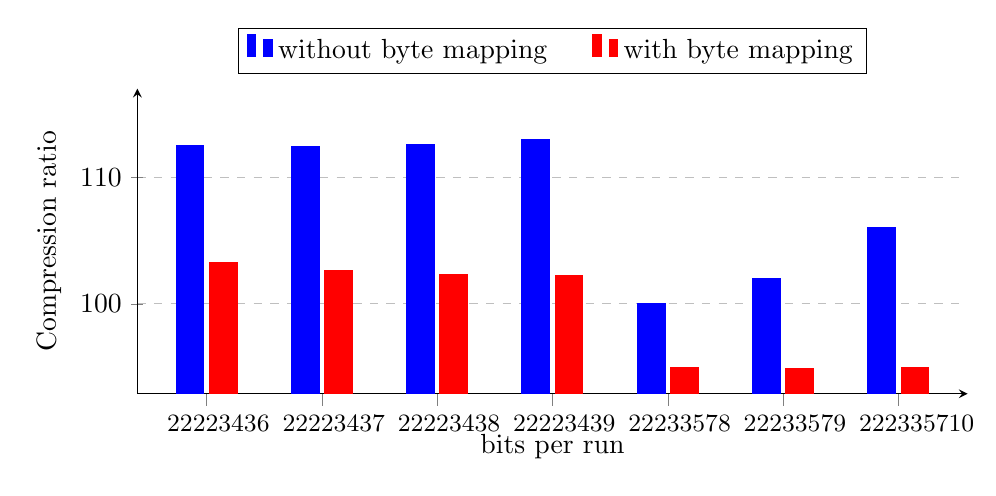
\begin{tikzpicture}
\begin{axis}[
width=\textwidth,
height=0.45\textwidth,
axis x line=center,
axis y line=left,
xlabel={bits per run},
ylabel={Compression ratio},
symbolic x coords={22223436,22223437,22223438,22223439,22233578,22233579,222335710},
x tick label style={font=\small,text width=1cm,align=center},
xtick=data,
x label style={at={(axis description cs:0.5,-0.1)},anchor=north},
enlargelimits=true,
ymax=115,
	legend style={
	at={(0.5,1.2)},
	anchor=north,
	legend columns=-1,
	/tikz/every even column/.append style={column sep=0.5cm}
},	
ymajorgrids=true,
grid style=dashed,
ybar]
\addplot[color=blue,fill]
	coordinates {
		(22223436,112.55)(22223437,112.4)(22223438,112.6)(22223439,113)(22233578,100)(22233579,102)(222335710,106)
	};
\addplot[color=red,fill]
coordinates {
	(22223436,103.3)(22223437,102.6)(22223438,102.3)(22223439,102.25)(22233578,95)(22233579,94.9)(222335710,95)
};
	\legend{without byte mapping,with byte mapping}
\end{axis}
\end{tikzpicture}
%}
%\end{scaletikzpicturetowidth}
\caption{Byte mapping and varying maximum run lengths.}
\label{fig:2:Byte mapping and varying maximum run lengths}
\end{figure}

\par{
Using this combined approach a real compression was achieved for the corpus instead of just one very specific file. The combination of 2 bits for the most insignificant bits, 3 for the fourth and fifth most insignificant bit 5 for the sixths most one, 7 bits for the second most significant bit and 9 bits for the most significant one yielded the overall best results with 94.9\% of its original size and 7.59 \textit{bps} as shown in Figure \ref{fig:2:Byte mapping and varying maximum run lengths}. Some files got a little smaller while other files still expanded which is only somewhat of an enhancement over regular RLE which performs really well on specific files. But on this corpus a slight reduction in size was achieved using preprocessing and a modified RLE.
\begin{table}[h]
	\centering
	\begin{tabular}{r|r|r|r|r}	
		file & size original & size encoded & ratio in \% & \textit{bps}\\
		\hline
bib & 111261 & 111579 & 100.29 & 8.02 \\
book1 & 768771 & 669578 & 87.10 & 6.97 \\
book2 & 610856 & 551757 & 90.33 & 7.23 \\
geo & 102400 & 144974 & 141.58 & 11.33 \\
news & 377109 & 363010 & 96.26 & 7.70 \\
obj1 & 21504 & 30166 & 140.28 & 11.22 \\
obj2 & 246814 & 340165 & 137.82 & 11.03 \\
paper1 & 53161 & 50074 & 94.19 & 7.54 \\
paper2 & 82199 & 71747 & 87.28 & 6.98 \\
pic & 513216 & 408136 & 79.53 & 6.36 \\
progc & 39611 & 38490 & 97.17 & 7.77 \\
progl & 71646 & 63765 & 89.00 & 7.12 \\
progp & 49379 & 46093 & 93.35 & 7.47 \\
trans & 93695 & 94729 & 101.10 & 8.09 \\
		\hline
		all files & 3145718 & 2988359 & 94.99 & 7.59
	\end{tabular}
	\caption{Calgary Corpus encoded with vertical reading, byte remapping, using bits per run (2, 2, 3, 3, 3, 4, 5, 8).}
\label{tab:t43 Calgary Corpus encoded with vertical reading, byte remapping and varying bits per run}
\end{table}
}

\section{Applying a Burrows-Wheeler-Transformation}
\par{
Another possible preprocessing step which promised an improvement is the mentioned Burrows-Wheeler-Transformation from Section \ref{ch:Principles of compression:sec:Other:subSec:bwt}, applied to all RLE implementations. Initially very simple transformation implementation was chosen, working by adding additional start and stop symbols to the input string (0x02 as STX, start of text and 0x03 as ETX, end of text). Some basic testing and playing around worked great but later on it revealed some major issues. For example the Calgary Corpus consists of more than text, in fact the files geo, obj1, obj2 and pic contain some binary data including the symbols STX or ETX, so we wont be able to apply the transformation to these. Another shortcoming was the very poor time complexity of almost $O (n^2)$ because under the hood, it uses a dual pivot Quick-sort algorithm from the JDK 11, which is typically faster than traditional one pivot Quick-sort. This algorithm offers $\Theta (n \: log(n))$ average time complexity but in the worst case, its time complexity is still cubic. This problem was partially solved by reading the input data in parts and performing the transformation on each part, resulting in a much smaller length $n$ and thus better run time at the expense of a slightly worse transformation result. As all chunks are individual transformations, they can also be computed in parallel.

\begin{table}[h]
	\centering
	\begin{tabular}{r|r|r}	
		bits per rle number & ratio in \% & \textit{bps}\\
		\hline
		3 & 95.41 & 7.63\\
		2 & 91.39 & 7.31 \\
	\end{tabular}
	\caption{Initial BWT implementation on byte wise RLE.}
	\label{tab:t11 Simple Burrows Wheeler Transformation on byte wise RLE}
\end{table}
}
\par{
While it was only applicable to textual data and very slow, even when divided into smaller parts and computed in parallel, it improved the overall results of byte wise RLE by 16\% to a compression ratio of slightly over 7 \textit{bps} as Table \ref{tab:t11 Simple Burrows Wheeler Transformation on byte wise RLE} depicts, which seemed like a good start. Regular binary RLE did not really benefit from this transformation as expected but on vertical interpretation, consecutive characters result in successive bits on every significance. Still this implementation had to be dropped and switched against one that could handle arbitrary input to be able to transform all files. This time all files could be processed and the resulting compression with byte wise RLE improved further as shown in table \ref{tab:t12 Burrows Wheeler Transformation on byte wise RLE}.
\begin{table}[h]
	\centering
	\begin{tabular}{r|r|r}	
		bits per rle number & ratio in \% & \textit{bps}\\
		\hline
		3 & 91.62 & 7.33\\
		2 & 89.46 & 7.15
	\end{tabular}
	\caption{Burrows Wheeler Transformation on byte wise RLE.}
	\label{tab:t12 Burrows Wheeler Transformation on byte wise RLE}
\end{table}
}

\par{
In general a Burrows-Wheeler-Transformation should also increase the runs in the implementation of Section \ref{ch:Analysis:sec:Improvements by Preprocessing:subSec:vertReading} and \ref{ch:Analysis:sec:Improvements by Preprocessing:subSec:byteRemapping} so those preprocessing steps were also applied in combination. To do so, it was first swapped against a sufficient implementation provided by a paper from M. Burrows and D. J. Wheeler \cite{Burrows94} from 1994. Their method is also the one described in Section \ref{ch:Analysis:sec:Improvements by Preprocessing:subSec:bwt} and could handle arbitrary input but it also had some downsides like the additional index $I$ of the transformation, which had to be persisted as well. The major downside of this implementation is the at least quadratic time complexity which made it still rather slow with increasing sizes of chunks, so again the input had to be spliced into small parts. If chunks exceeded a length of more than one kilobyte it became unacceptably slow even though it strongly improved the transformation results so most of the time and in Table \ref{tab:t12 Burrows Wheeler Transformation on byte wise RLE} and \ref{tab:t13 Modified Burrows Wheeler Transformation on byte wise RLE} the transformation was performed on chunks of size 512 byte. To overcome this degradation of the original algorithm and the necessity of saving  additional indices, the implementation had to be swapped once more against one that was first described in \cite{Burrows-linear-time} int eh year 2009 which claimed to perform in linear time complexity.
}
\par{
In form of the C library \href{https://code.google.com/archive/p/libdivsufsort}{libdivsufsort} a working implementation of BWTS was found, the bijective Burrows-Wheeler-Scott-Transformation described in \cite{DBLP:journals/corr/abs-1201-3077}. This kind of Burrows-Wheeler-Transformation does not require additional information, no start and stop symbols or an index of its original position. Briefly, it does not construct a matrix of all cyclic rotations, instead it is computed with a suffix array sorted with DivSufSort \cite{LibDivSufSort}, closer described in the paper \cite{DBLP:journals/corr/abs-1710-01896}, which is the fastest currently known method of constructing the transformation. To use it properly the code was ported to Kotlin but there are also ports of this library in Java and Go available which are recommended because the original code is neither documented nor readable and the functionality can easily be used via a dependency.
}
\par{
The simple binary RLE did not really benefit from this transformation which has to be expected, because it generates repetitions of bytes, but if a byte needs many short runs it will still expand in size because the average runs are not that much influenced. For example just the letter \enquote{e} needs 6 different runs, no matter on which position or surrounded by what letters. The byte wise implementation on the other hand did very strongly benefit from this transformation, it will always create longer runs of equal bytes. Swapping the implementation of the Burrows-Wheeler-Transformation resulted in way better results, the simple byte wise RLE achieving compression ratios around $59 \%$ of its original size while using 4 bits per run, see Table \ref{tab:t13 Modified Burrows Wheeler Transformation on byte wise RLE}. This was mainly because of the longer repetitions possible after the transformation was performed on the whole input instead of small chunks. Interestingly, average runs of characters increased so much, that 4 bits per run achieved the maximum result. Another reason for this vast improvement compared to the old implementations is the lack of additional information needed to store because we do no longer need to store the transformation index of every chunk or additional characters.
	\begin{table}[h]
		\centering
		\begin{tabular}{r|r|r}	
			bits per rle number & ratio in \% & \textit{bps}\\
			\hline
			8 & 74.42 & 5.95\\
			7 & 69.90 & 5.59\\
			6 & 65.58 & 5.24\\
			5 & 61.71 & 4.93\\
			4 & 58.98 & 4.71\\
			3 & 59.18 & 4.73\\
			2 & 67.69 & 5.41
		\end{tabular}
		\caption{Modified Burrows Wheeler Transformation on byte wise RLE.}
		\label{tab:t13 Modified Burrows Wheeler Transformation on byte wise RLE}
	\end{table}
}
\par{
Working on the whole input data and no longer on small chunks, this BWTS generates extreme long runs of identical byte values, which in turn enhances the performance of the byte wise RLE vastly. If we take a closer look we can see in Table \ref{tab:t14:Calgary Corpus encoded with byte wise RLE after a Burrows-Wheeler-Transformation} that all files have a compression ratio below $100\%$ while the total size is nearly reduced to half. The file \textit{geo} is still close to uncompressed but half of the files only need less than 5 \textit{bps}. The file \textit{pic} is still the best compressible with only 2.12 \textit{bps}.
\begin{table}[h]
	\centering
	\begin{tabular}{r|r|r|r|r}	
		file & size original & size encoded & compression & \textit{bps}\\
		\hline
bib & 111261 & 59285 & 53.28 & 4.26 \\
book1 & 768771 & 590879 & 76.86 & 6.15 \\
book2 & 610856 & 374742 & 61.35 & 4.91 \\
geo & 102400 & 101192 & 98.82 & 7.91 \\
news & 377109 & 246047 & 65.25 & 5.22 \\
obj1 & 21504 & 16467 & 76.58 & 6.13 \\
obj2 & 246814 & 126626 & 51.30 & 4.10 \\
paper1 & 53161 & 34130 & 64.20 & 5.14 \\
paper2 & 82199 & 56507 & 68.74 & 5.50 \\
pic & 513216 & 136074 & 26.51 & 2.12 \\
progc & 39611 & 24312 & 61.38 & 4.91 \\
progl & 71646 & 31466 & 43.92 & 3.51 \\
progp & 49379 & 20862 & 42.25 & 3.38 \\
trans & 93695 & 32835 & 35.04 & 2.80 \\
\hline
all files & 3145718 & 1855520 & 58.98 & 4.71
	\end{tabular}
	\caption{Calgary Corpus encoded with byte wise RLE after a Burrows-Wheeler-Transformation with 4 bit per run.}
	\label{tab:t14:Calgary Corpus encoded with byte wise RLE after a Burrows-Wheeler-Transformation}
\end{table}
}
\par{
There should still be room for some optimizations because as seen in Section \ref{ch:Conceptual Design:sec:var lengths}, the remapping of the input resulted in longer runs on the higher order bits and the vertical interpretation made it possible to encode different sections with different maximum run lengths. It was expected that applying the Burrows-Wheeler-Transformation to the vertical encoding variant should improve its efficiency as much as the byte wise RLE did benefit, which turned out to be wrong. The vertical interpretation did indeed perform at its best when applying the BWTS and the mapping but it did not outperform the combination of BWTS and byte wise RLE which is kind of expected because the transformation creates repetitions on byte level.

\begin{figure}[h]
	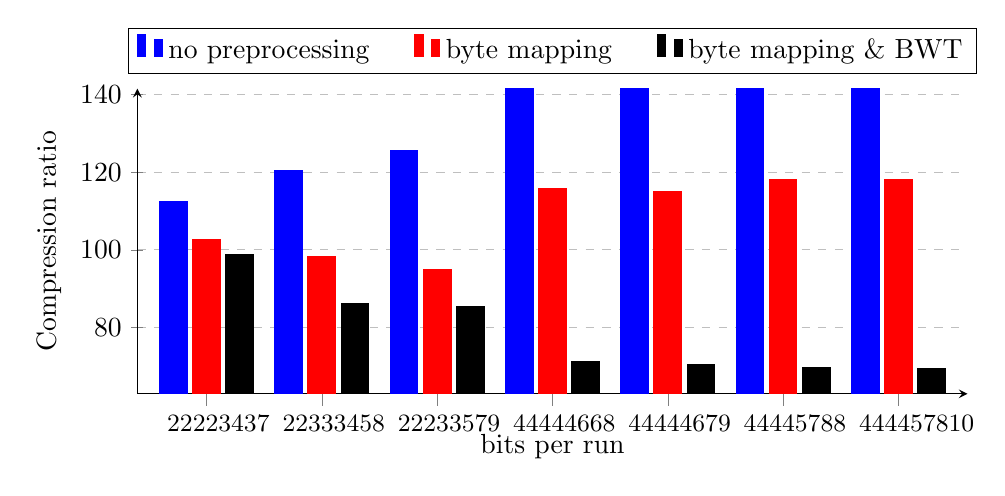
\begin{tikzpicture}
	\begin{axis}[
	width=\textwidth,
	height=0.45\textwidth,
	axis x line=center,
	axis y line=left,
	xlabel={bits per run},
	x label style={at={(axis description cs:0.5,-0.1)},anchor=north},
	ylabel={Compression ratio},
	symbolic x coords={22223437,22333458,22233579,44444668,44444679,44445788,444457810},
	x tick label style={font=\small,text width=1cm,align=center},
	xtick=data,
	enlargelimits=true,
	ymax=135,
	legend style={
	at={(0.5,1.2)},
	anchor=north,
	legend columns=-1,
	/tikz/every even column/.append style={column sep=0.5cm}
	},	
	ymajorgrids=true,
	grid style=dashed,
	ybar
	]
	\addplot[color=blue,fill]
	coordinates {
		(22223437,112.4)(22333458,120.4 )(22233579,125.6)(44444668,147.2)(44444679,151.3)(44445788,159.7)(444457810,160.8)
		};
	\addplot[color=red,fill]
	coordinates {
		(22223437,102.6)(22333458,98.2 )(22233579,94.99)(44444668,115.7)(44444679,115.1)(44445788,118)(444457810,118)
	};
	\addplot[color=black,fill]
	coordinates {
		(22223437,98.8)(22333458,86.1 )(22233579,85.3)(44444668,71.2)(44444679,70.3)(44445788,69.6)(444457810,69.4)
	};
	\legend{no preprocessing,byte mapping,byte mapping \& BWT}
	\end{axis}
	\end{tikzpicture}
	%}
	%\end{scaletikzpicturetowidth}
	\caption{Byte mapping and varying maximum run lengths, all preprocessing steps.}
	\label{fig:3:Different run lengths with and without transformations}
\end{figure}

\par{
\begin{table}[h]
	\centering
	\begin{tabular}{r|r|r|r|r}	
		file & size original & size encoded & ratio in \% & \textit{bps}\\
		\hline
		bib & 111261 & 73843 & 66.37 & 5.31 \\
		book1 & 768771 & 570348 & 74.19 & 5.94 \\
		book2 & 610856 & 409639 & 67.06 & 5.36 \\
		geo & 102400 & 145950 & 142.53 & 11.40 \\
		news & 377109 & 275396 & 73.03 & 5.84 \\
		obj1 & 21504 & 27023 & 125.66 & 10.05 \\
		obj2 & 246814 & 213392 & 86.46 & 6.92 \\
		paper1 & 53161 & 37344 & 70.25 & 5.62 \\
		paper2 & 82199 & 56490 & 68.72 & 5.50 \\
		pic & 513216 & 227914 & 44.41 & 3.55 \\
		progc & 39611 & 28275 & 71.38 & 5.71 \\
		progl & 71646 & 38144 & 53.24 & 4.26 \\
		progp & 49379 & 27029 & 54.74 & 4.38 \\
		trans & 93695 & 49314 & 52.63 & 4.21 \\
		\hline
		all files & 3145718 & 2184197 & 69.43 & 5.55
	\end{tabular}
	\caption{Calgary Corpus encoded, byte mapping and a BWTS as preprocessing, using bits per run (4, 4, 4, 4, 5, 7, 8, 10).}
	\label{tab:t5:Calgary Corpus encoded, all preprocessing steps, using bits per run: 4, 4,4, 4, 5, 7, 8, 10}
\end{table}

\par{
One last option was the encoding of the lowest significant bits with another, more suited scheme like Huffman encoding was tried out but with rather poor results. It was found that encoding the last or the last few rows seen in \ref{ch:Analysis:sec:Improvements by Preprocessing:subSec:vertReading} with did not improve overall results and it was therefore discarded. This might be related to the high improvement in RLE after a Burrows-Wheeler-Transformation and other factors like additional overhead because the mapping of the Huffman encoding has to be persisted with the encoded data. But the idea of combining the RLE methods with Huffman encoding still stuck around and was picked up again later on in a modified way in Section \ref{ch:Conceptual Design:sec:Postprocessing}. No further attempts to add or improve preprocessing steps of this kind were made, instead the results were analyzed and compared with other results in Section \ref{ch:Evaluation}.
}
%% ==============================
\section{Huffman Encoding of the RLE Runs}
%% ==============================
\label{ch:Conceptual Design:sec:Postprocessing}
\par{
Encoding of run lengths using Huffman codes was implemented, similar to the Fax Transmission Standard mentioned in Section \ref{ch:Principles of compression:sec:Run Length Encoding:subSec:History}, but in a dynamic way instead of predefined static codes. This idea was also used by Burrows and Wheeler in their paper \cite{Burrows94} but instead of RLE they combined a Move to Front Coder with their transformation and then encoded the result using Huffman codes. This way it would be possible to encode more frequent results of the Move-to-Front Encoder or the Run Length Encoder could be encoded into shorter codes and thus save even more space. This step is not really considered preprocessing anymore but could improve the compression furthermore, however the benefit of Huffman encoding is the possibility to output codes of varying length as described in Section \ref{ch:Principles of compression:sec:Huffman Coding}. Combining the binary or vertical encoded RLE with a Huffman encoder would be a huge benefit, because as of now the algorithm needs to output a number of bits for each number to encode. Combined, the more frequent short runs of 1 or 2 can be encoded into shorter Huffman codes which should increase the overall compression algorithm. In general it was assumed that there was no longer a benefit in using different maximum run lengths on bits of different significance, because a run of any given length is going to be encoded with a Huffman code, not with just a fixed amount of bits. To reverse the Huffman encoding, the Huffman tree has to be persisted into the file as well.
	\begin{table}[H]
		\centering
		\begin{tabular}{r|r|r|r|r}	
			file & size original & size encoded & ratio in \% & \textit{bps}\\
			\hline
bib & 111261 & 44156 & 39.69 & 3.17 \\
book1 & 768771 & 340279 & 44.26 & 3.54 \\
book2 & 610856 & 243092 & 39.80 & 3.18 \\
geo & 102400 & 63006 & 61.53 & 4.92 \\
news & 377109 & 173207 & 45.93 & 3.67 \\
obj1 & 21504 & 14405 & 66.99 & 5.36 \\
obj2 & 246814 & 119957 & 48.60 & 3.89 \\
paper1 & 53161 & 24917 & 46.87 & 3.75 \\
paper2 & 82199 & 35939 & 43.72 & 3.50 \\
pic & 513216 & 82136 & 16.00 & 1.28 \\
progc & 39611 & 18890 & 47.69 & 3.82 \\
progl & 71646 & 24649 & 34.40 & 2.75 \\
progp & 49379 & 17416 & 35.27 & 2.82 \\
trans & 93695 & 31235 & 33.34 & 2.67 \\
			\hline
			all files & 3145718 & 1237380 & 39.33 & 3.14
		\end{tabular}
		\caption{Calgary Corpus encoded with vertical reading, byte mapping and a BWTS as preprocessing, using Huffman encoding for all counted runs, 8 bit per run.}
		\label{tab:t6:Calgary Corpus encoded, all preprocessing steps, using Huffman encoding for all counted runs}
	\end{table}
}
\par{
This combination of vertical encoding with byte remapping and the sophisticated BWTS as preprocessing steps so far best results have been found. Although, at first glance it was suggested to eliminate the maximum run restriction to possibly compress all bits of one significance into a single Huffman code, it turned out to be most efficient if the run length process is limited to 8 bits per run. This way still a total of 255 bits of same significance can be encoded into one during the RLE step, but there will be only a maximum of 256 different Huffman codes generated. Average Huffman code length will be significantly shorter. Also it makes no sense to use different maximum run lengths for bits of different significance, because there will still be one Huffman code for each different run value. The results are depicted in Table \ref{tab:t6:Calgary Corpus encoded, all preprocessing steps, using Huffman encoding for all counted runs}.
}
\section{Summary}
\par{
Using a composition of preprocessing steps, another data interpretation in form of the vertical reading and optimal prefix codes as encoding due to the Huffman encoder, acceptable results have been achieved. Not only was there a reasonable compression for every file, the file \textit{pic} was compressed even better than before, although it is highly suited for the original proposed RLE. 
}
%%% Local Variables: 
%%% mode: latex
%%% TeX-master: "thesis"
%%% End: 
     % Entwurf
%%% implemen.tex
%% $Id: implemen.tex 61 2012-05-03 13:58:03Z bless $
%%

\chapter{Implementierung}
\label{ch:Implementierung}
%% ==============================
\ldots

%% ==============================
\section{Abschnitt 1}
%% ==============================
\label{ch:Implementierung:sec:Abschnitt1}

\ldots

%% ==============================
\section{Abschnitt 2}
%% ==============================
\label{ch:Implementierung:sec:Abschnitt2}

\ldots

%%% Local Variables: 
%%% mode: latex
%%% TeX-master: "thesis"
%%% End: 
    % Implementierung
%%% eval.tex
%% $Id: eval.tex 61 2012-05-03 13:58:03Z bless $

\chapter{Evaluation}
\label{ch:Evaluation}
%% ==============================

In this evaluation section, we explore how well the algorithm performs by looking at the performance and examining the decompositions. Our primary interest lies in two aspects, the size of the factors contributing to the decomposition and the coverage of final states by each factor. Through this analysis, we aim to gauge the algorithm's effectiveness in generating meaningful decompositions. This evaluation is pivotal for understanding the algorithm's capability to produce concise and relevant factors, providing insights into the temporal structure of the give labels. For this purpose, the complete f2f dataset was evaluated, described in Section \ref{ch:prelimiaries:real-world-data} consisting of 62 Temporal graphs with 20 to 56 edges each, ignoring loop edges. In total there are 3321 edges with a combined label length of around 2.3 million giving an average label length of 6993. Please not that the data sets represent people looking at each other, a directed edge from node $u$ to $v$ indicates participant $u$ looks at participant $v$ therefore only one edge label at a given time step $t$ has its value set, $\tau(e)[t] = 1$ for exactly one outgoing edged of $u$. This is also visible in the data as only 13.4\% of values in the labels is set to 1 over all the labels.

\section{Performance Evaluation}
Although performance was not the main focus of the implementation and evaluation, generating \orDecomp for the complete dataset is reasonable fast with around 3 seconds if using the maximal divisors or the greedy approach. The Fourier-transformation takes a lot of additional time for cleaning multiples of a factor as well as replacing factors with multiple set values with a set of factors with only one set value, causing it to run for 1 minute and 45 seconds. All benchmarks were performed on an AMD Ryzen 5 2600X six core processor (12 threads) with a 3.6 GHz base clock and a 4.2 GHz boost clock speed. For memory, 16GB 3200MHz ram and a Samsung evo ssd was used for persistent storage.
\begin{table}[h]
	\begin{tabular}{l|lll}
		 & MaxDivisors & GreedyShortFactors & FourierTransform  \\
		\hline
		 OR-Decomposition & 3.12 & 3.47 & 105 \\
		 AND-Decomposition & 9.85 & 24.83 & - \\
		 	
	\end{tabular}
	\caption{Decomposition time in seconds [s] for complete dataset}
	\label{tab:eval-performance}
\end{table}
It is to not that the \andDecomp is expected to be slower because of considerably greater amount of zeros in the data set as well as the modification to the cover finding algorithm. While with an \orDecomp, each additional factor can only remove outliers, in an \andDecomp an additional factor can also add new outliers. Because of that, the current outliers of a decomposition must be recalculated considering all factors. The Fourier-transform method again increases the amount of factors per cover, which hurts performance. Also it is not implemented for \andDecomp as it is not considered reasonable, since a human would still need to look at all factors since it is an \andDecomp.

\section{Decomposition Evaluation}
Moving on to the decomposition evaluation, we validate each method separately and then compare them against each other. We also benchmark \andDecomp and \orDecomp. To get an insight on how well a particular decomposition method is performing, decompose the whole data-set and then plot each factor of each decomposition by its relative size compared to the original \DFA size and the relative amount of covered values of the \DFA by this factor.
\begin{figure}[t]
	\begin{minipage}[h]{0.49\linewidth}
		\centering
		OR-decomposition
		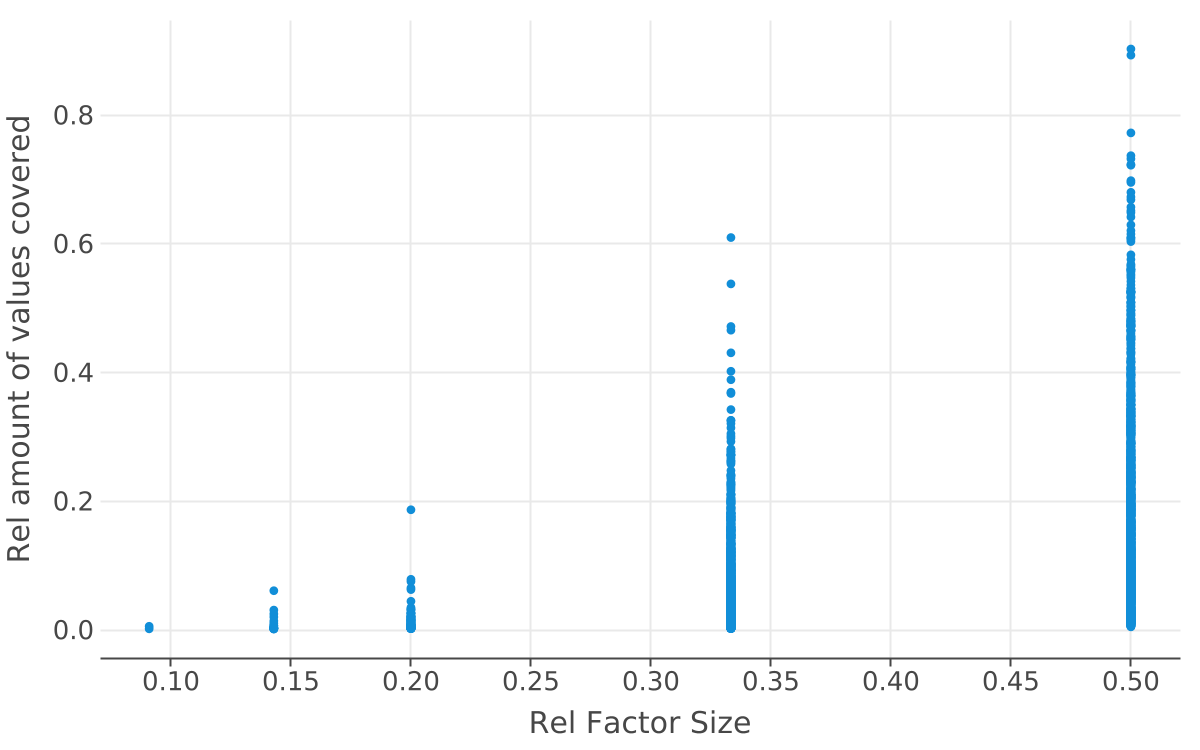
\includegraphics[width=\linewidth]{../plots/point-plots/MAX_DIVISORS-OR-all-relative-values-by-factor-size.png}
	\end{minipage}
	\begin{minipage}[h]{0.49\linewidth}
		\centering
		AND-decomposition
		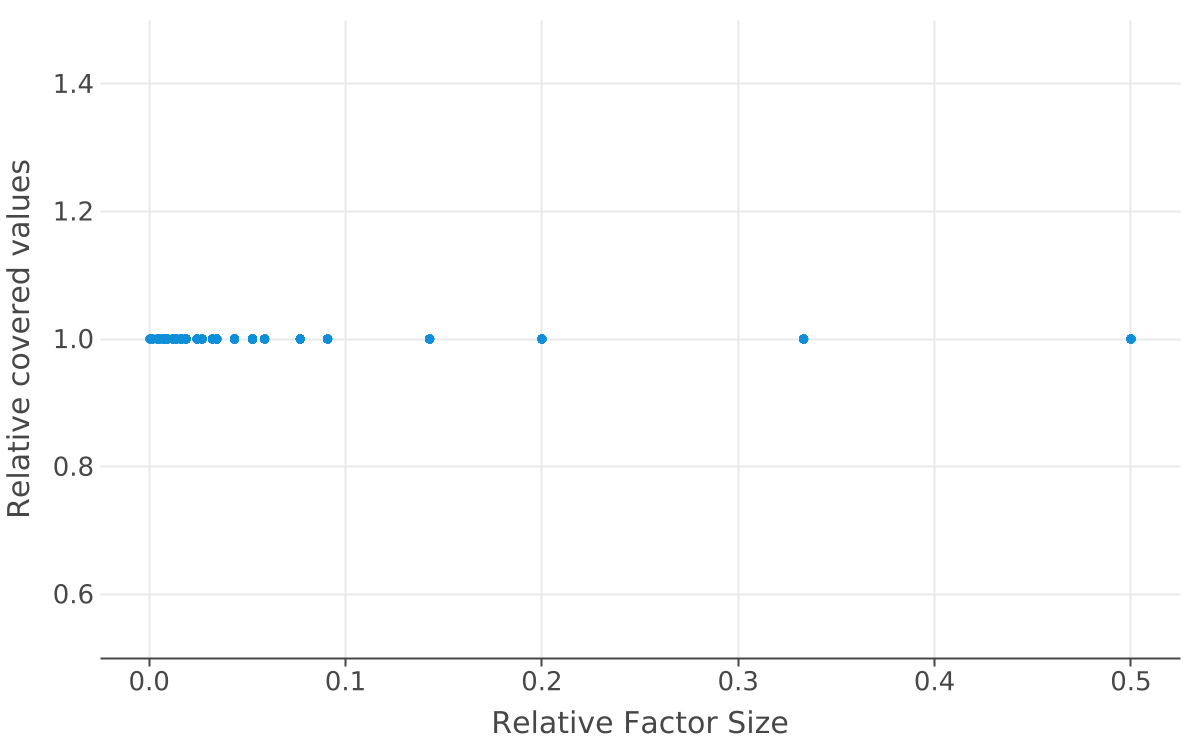
\includegraphics[width=\linewidth]{../plots/point-plots/MAX_DIVISORS-AND-all-relative-values-by-factor-size.png}
	\end{minipage}
	\caption{Relative amount of covered values by relative factor size}
	\label{fig:eval:max-divisor-all-factors}
\end{figure}

\subsection{Maximal Divisor Decomposition Evaluation}
Decomposing with the Maximal Divisor method implemented as described in Section \ref{ch:Implementation:max-divisor} was used first for decomposing the complete dataset. Analyzing the resulting decompositions and plotting each factor $B_i$ of each decomposition of a \DFA $A$ by its size relative to the original $\frac{|B_i|}{|A|}$ with its relative amount of covered final states from $A$, the precision up to that factor. The results are shown in Figure \ref{fig:eval:max-divisor-all-factors} and it clearly shows that the \orDecomp finds factors, but there are less factors in the decompositions and they cover fewer values than the comparable \andDecomp.
\begin{figure}[h]
	\begin{minipage}[h]{0.49\linewidth}
		\centering
		OR-decomposition
		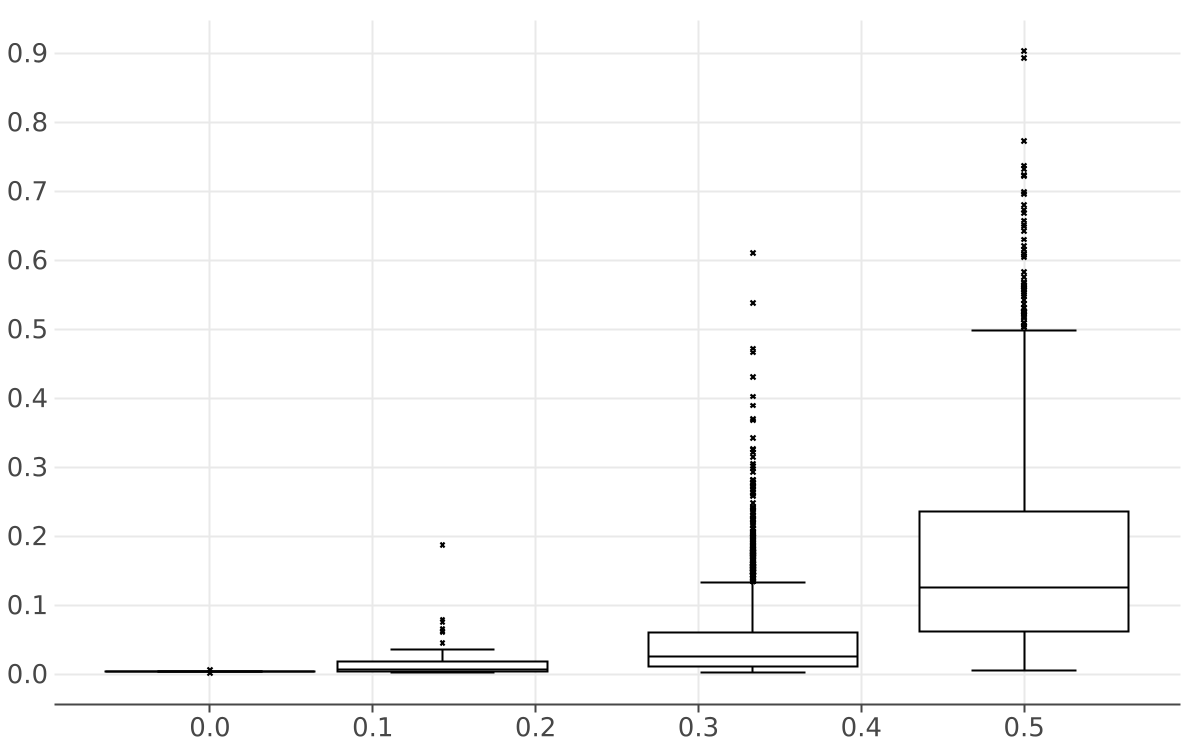
\includegraphics[width=\linewidth]{../plots/box-plots/MAX_DIVISORS-OR-all-relative-values-by-factor-boxplot-dist.png}
	\end{minipage}
	\begin{minipage}[h]{0.49\linewidth}
		\centering
		AND-decomposition
		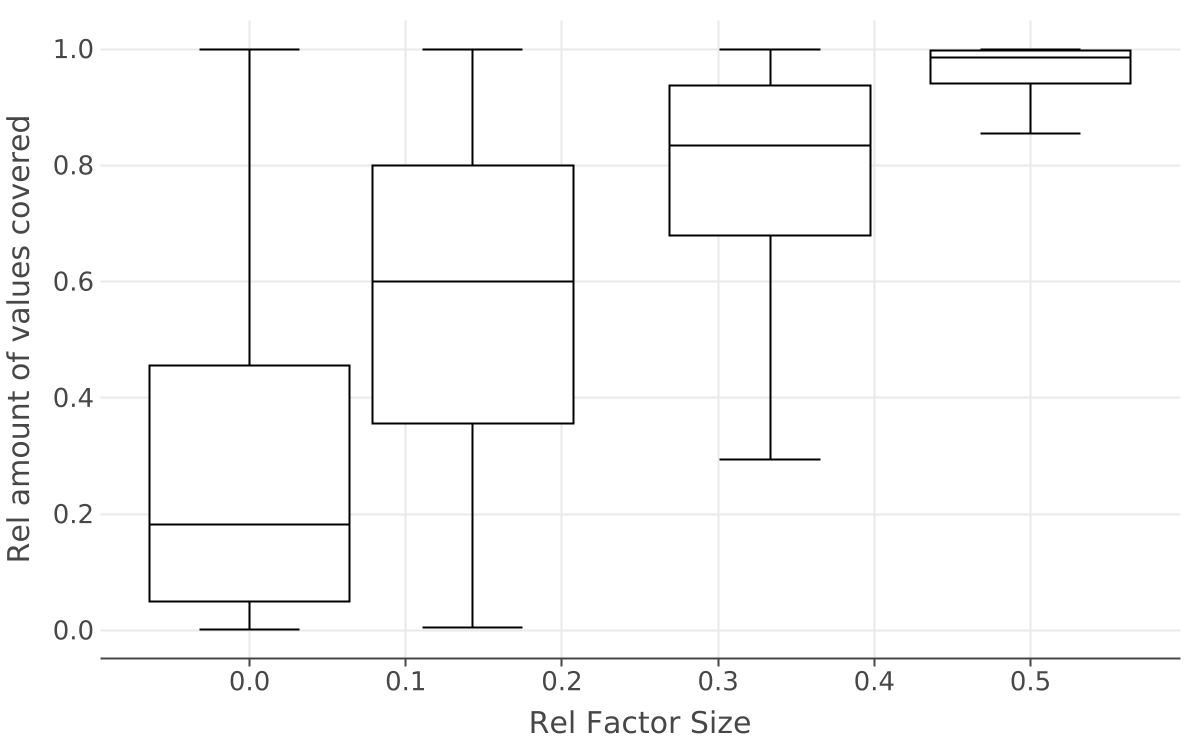
\includegraphics[width=\linewidth]{../plots/box-plots/MAX_DIVISORS-AND-all-relative-values-by-factor-boxplot-dist.png}
	\end{minipage}
	\caption{Relative amount of covered values by relative factor size (MaxDivisors)}
	\label{fig:eval:max-divisor-all-factors-box-plot}
\end{figure}
A lot of data-points collapse onto a single x value since they are grouped by their relative size, not their absolute. For the \andDecomp there are many values scattered around a small relative factor size. To get some more insight into the distribution, a box plot is also provided in Figure \ref{fig:eval:max-divisor-all-factors-box-plot}. Here, the same x and y values are chosen but the values are aggregated such that if a x value is to close to another, their data points gets merged. The \orDecomp shows that even with a relative factor size of $\frac{1}{2}$ which is the largest possible factor, the median over all these factors only cover 10\% of the target \DFA. There are some outliers with $\frac{1}{3}$ or $\frac{1}{2}$ the original size which cover already up to 60-80\% of the original \DFA but they are outliers and most of the \orDecomp found by using the maximal divisors cover almost nothing of the original, especially the short factors. For the \andDecomp a lot of the small relative factor sizes have to be aggregated in order to visualize them as box-plots, so if a relative factor size value is less than $\frac{1}{20}$ away from a previous data-point, they become one distribution. Notably, factors of size between $\frac{1}{12}$ and $\frac{1}{5}$ stretch over the entire range of relative covered values in the decomposition. With $\frac{1}{6}$ relative factor size, the \andDecomp already covered more than 50\% of a given \DFAs final states.

\subsection{Greedy Short Factor Decomposition Evaluation}
Looking at the novel greedy approach for finding short factors, a similar picture becomes evident. We find more factors and some better ones as before when using just the maximal divisors as potential factor sizes, but some factor size data points from Figure \ref{fig:eval:greedy-short-factors-all-factors} only have a single factor with that relative size. Although there are now more factors present overall, the short factors found, only cover at most 20\% of the final states of the \DFA they compose.
\begin{figure}[h]
	\begin{minipage}[h]{0.49\linewidth}
		\centering
		OR-decomposition
		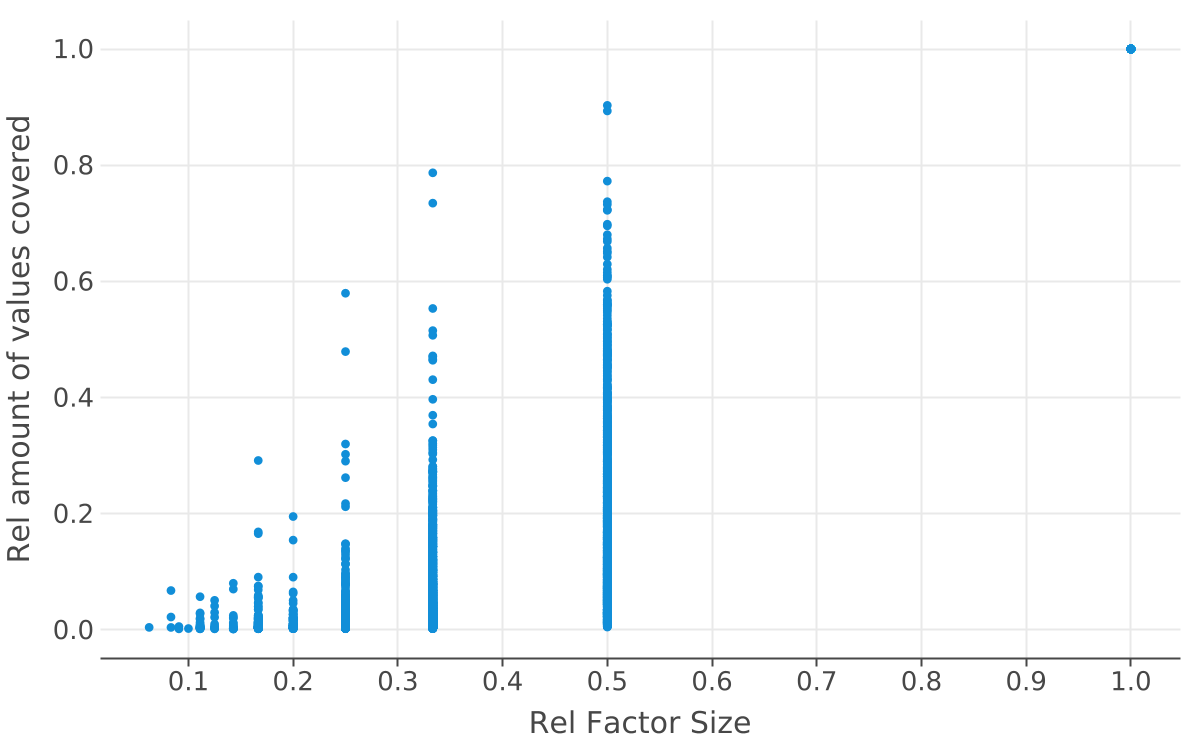
\includegraphics[width=\linewidth]{../plots/point-plots/GREEDY_SHORT_FACTORS-OR-all-relative-values-by-factor-size.png}
	\end{minipage}
	\begin{minipage}[h]{0.49\linewidth}
		\centering
		AND-decomposition
		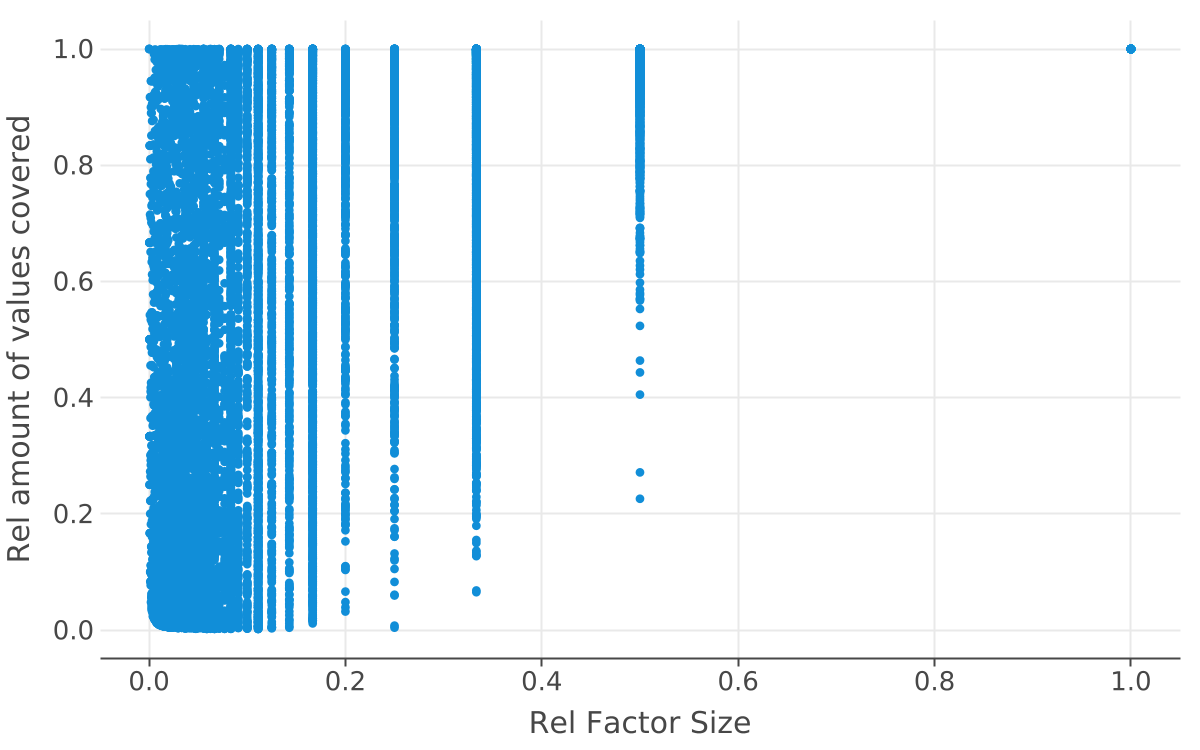
\includegraphics[width=\linewidth]{../plots/point-plots/GREEDY_SHORT_FACTORS-AND-all-relative-values-by-factor-size.png}
	\end{minipage}
	\caption{Relative amount of covered values by relative factor size}
	\label{fig:eval:greedy-short-factors-all-factors}
\end{figure}
As Figure \ref{fig:eval:greedy-short-factors-all-factors-box-plot} shows, we find more factors and even some better outliers of the distribution, but the overall covered values stays very low. There are factors of relative size $\frac{1}{3}$ or $\frac{1}{2}$ which cover up to 80\% of the final states of their \DFA present, but the median over the distributions never exceed 16\%. 
\begin{figure}[t]
	\begin{minipage}[h]{0.49\linewidth}
		\centering
		OR-decomposition
		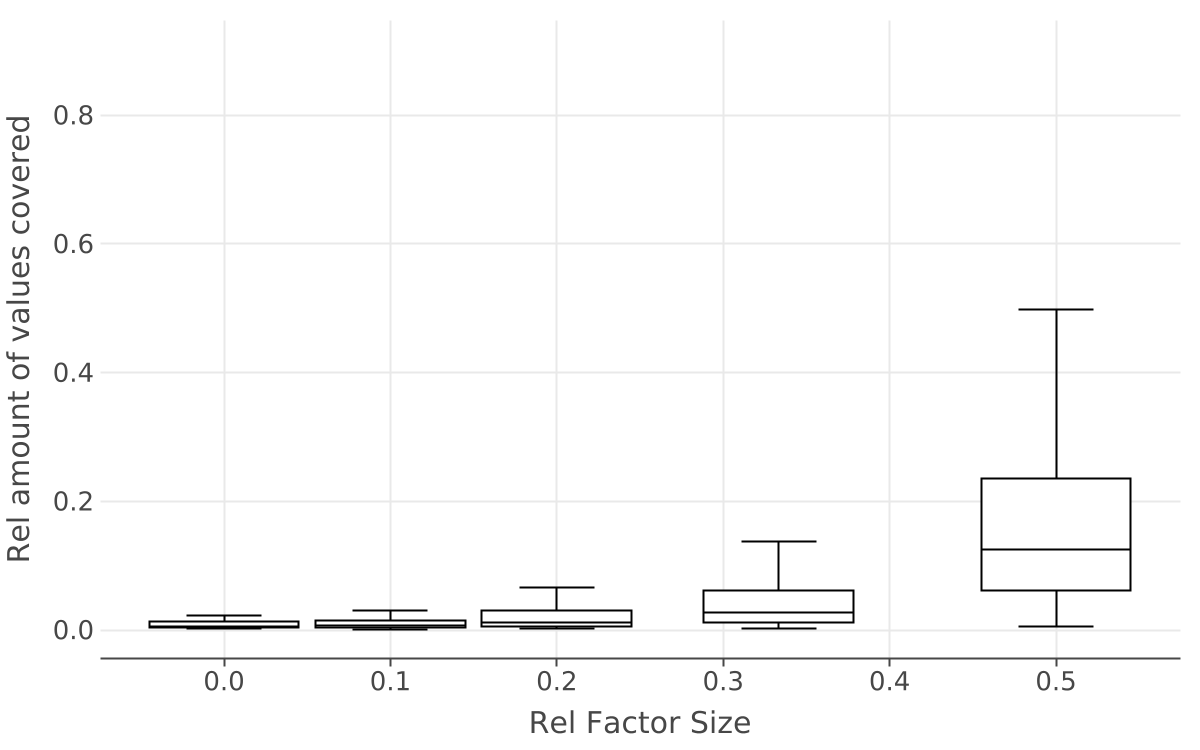
\includegraphics[width=\linewidth]{../plots/box-plots/GREEDY_SHORT_FACTORS-OR-all-relative-values-by-factor-boxplot-dist.png}
	\end{minipage}
	\begin{minipage}[h]{0.49\linewidth}
		\centering
		AND-decomposition
		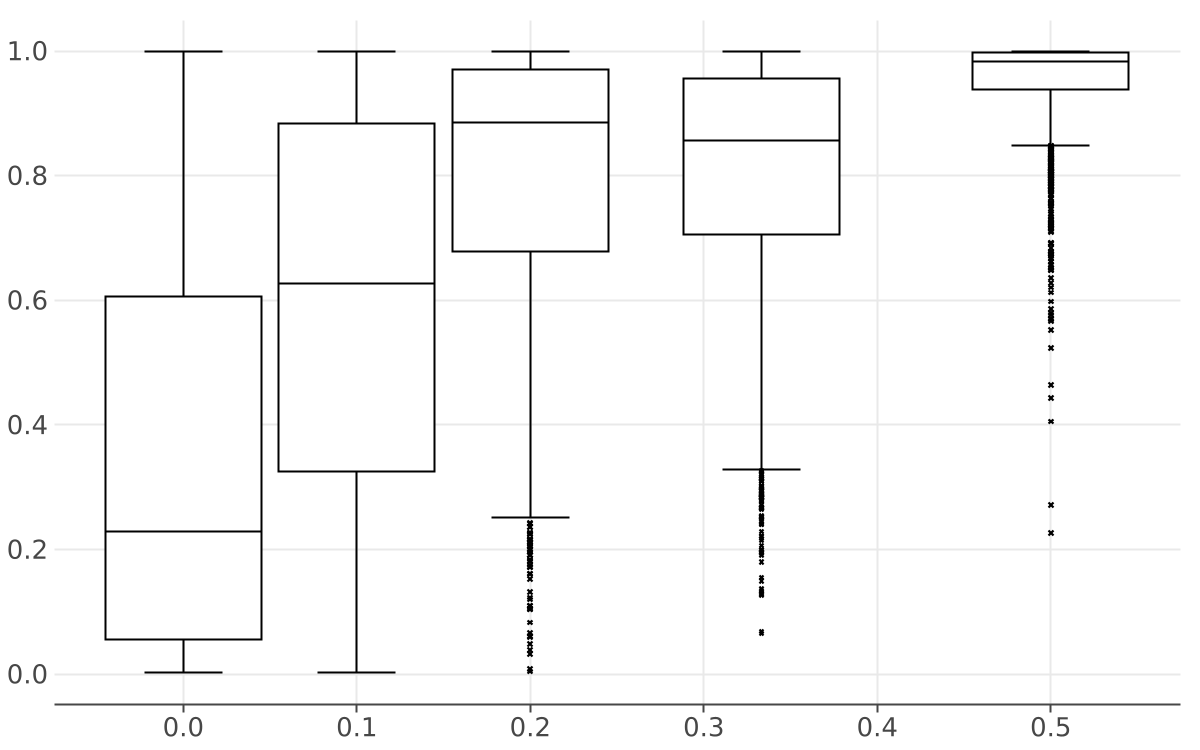
\includegraphics[width=\linewidth]{../plots/box-plots/GREEDY_SHORT_FACTORS-AND-all-relative-values-by-factor-boxplot-dist.png}
	\end{minipage}
	\caption{Relative amount of covered values by relative factor size (GreedyShorFactors)}
	\label{fig:eval:greedy-short-factors-all-factors-box-plot}
\end{figure}

TODO:elaborate

\newpage
\subsection{Fourier-Transform Decomposition Evaluation}
TODO: explain
\begin{figure}[h]
	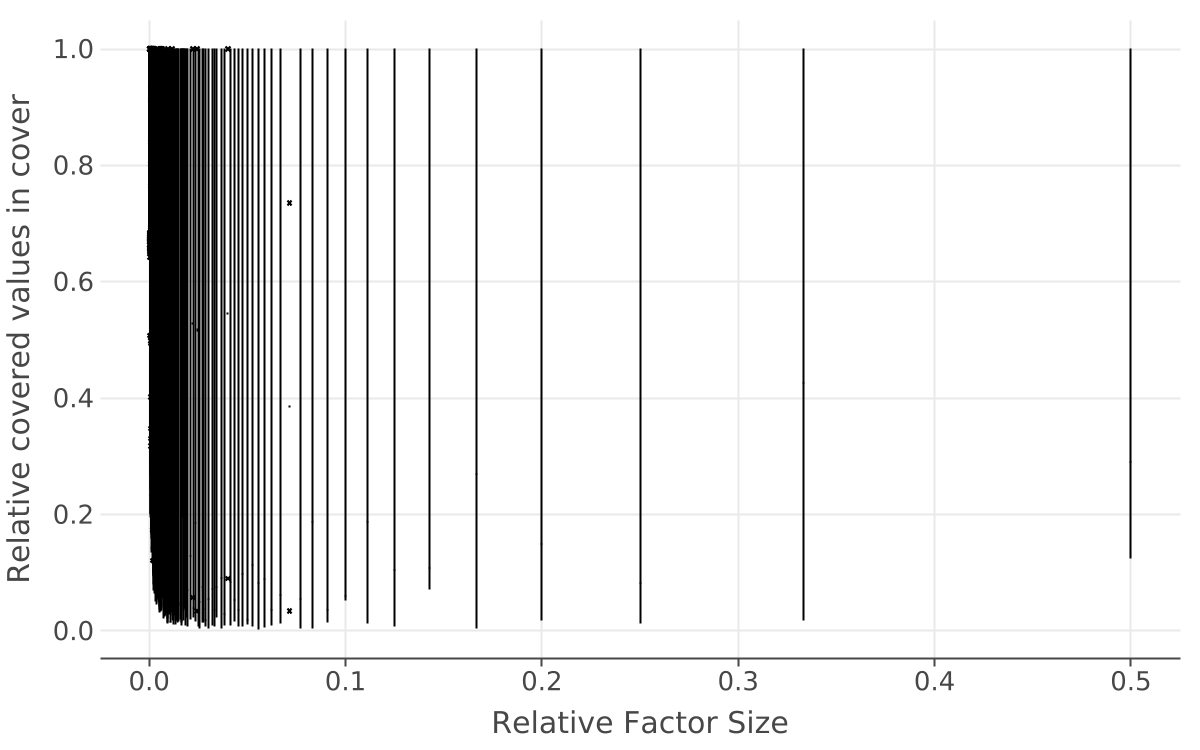
\includegraphics[width=\linewidth]{../plots/box-plots/FOURIER_TRANSFORM-OR-all-relative-values-by-factor-boxplot-outliers.png}
	\caption{Relative amount of covered values by relative factor size (FourierTransform)}
	\label{fig:eval:fourier-all-factors-box-plot}
\end{figure}

\newpage
\newpage
\section{Explainability Evaluation}
TODO: fix table, maybe remove median ? or precision in extra table as values are duplicated ?
\begin{table}[h]
	\begin{tabular}{ll||rrrrrr|rr|rrr}
		& & valid & good & ok &  \multicolumn{3}{c}{ds} & \multicolumn{2}{c}{precision} & \multicolumn{3}{c}{size}  \\
		& & & & & $\Sigma$ & a & m & avg & m & $\Sigma$ & avg & m\\
		\hline
		\hline
		\multirow{2}{*}{MaxDivisors} & $\cap$ & 182 & 1908 & 2670 & 490 & 0.14 & 0.11 &  0.86 & 0.93 & 7010 & 2.11 & 2 \\
		 & $\cup$ & 3 & 3 & 3 & 1300 & 0.39 & 0.33 & 0.08 & 0.03 & 3629 & 1.09 & 1 \\
		 \hline
		\multirow{2}{*}{GreedyShortFactors} & $\cap$ & 182 & 1908 & 2670 & 985 & 0.29 & 0.19 & 0.86 & 0.93 & 17247 & 5.19 & 3 \\
		& $\cup$ & 3 & 3 & 3 & 1396 & 0.42 & 0.33 & 0.08 & 0.03 & 4095 & 1.23 & 1 \\
		\hline
		FourierTransform & $\cup$ & 3 & 3 & 3 & 1654 & 0.49 & 0.33 & 0.08 & 0.03 & 4390 & 1.32 & 1 \\
	\end{tabular}
	\caption{Explainability metrics for different methods}
	\label{tab:eval-metric}
\end{table}

TODO: explain
%%% Local Variables: 
%%% mode: latex
%%% TeX-master: "thesis"
%%% End: 
        % Evaluation
%%% zusammenf.tex
%% $Id: zusammenf.tex 61 2012-05-03 13:58:03Z bless $
%%

\chapter{Diskussion und Ausblick}
\label{ch:fazit}
%% ==============================

(Keine Untergliederung mehr)

%%% Local Variables: 
%%% mode: latex
%%% TeX-master: "thesis"
%%% End: 
   	  % Diskussion und Ausblick

%% ++++++++++++++++++++++++++++++++++++++++++
%% Anhang
%% ++++++++++++++++++++++++++++++++++++++++++

\appendix
%\include{anhang_a}
%\include{anhang_b}

%% ++++++++++++++++++++++++++++++++++++++++++
%% Literatur
%% ++++++++++++++++++++++++++++++++++++++++++
%  mit dem Befehl \nocite werden auch nicht 
%  zitierte Referenzen abgedruckt

\cleardoublepage
\phantomsection
\addcontentsline{toc}{chapter}{\bibname}
%%
%%\nocite{*} % nur angeben, wenn auch nicht im Text zitierte Quellen 
           % erscheinen sollen
%\bibliographystyle{itmabbrv} % mit abgekürzten Vornamen der Autoren
\bibliographystyle{cpc} % abbrvnat unsrtnat
% spezielle Zitierstile: Labels mit vier Buchstaben und Jahreszahl
%\bibliographystyle{itmalpha}  % ausgeschriebene Vornamen der Autoren

\bibliography{thesis}

%% ++++++++++++++++++++++++++++++++++++++++++
%% Index
%% ++++++++++++++++++++++++++++++++++++++++++
\ifnotdraft{
\cleardoublepage
\phantomsection
\printindex            % Index, Stichwortverzeichnis
}

 %
 % Die folgende Erklärung ist für Diplomarbeiten Pflicht
 % (siehe Prüfungsordnung), für Studienarbeiten nicht notwendig
 \thispagestyle{empty}
%\vspace*{35\baselineskip}
%\hbox to \textwidth{\hrulefill}
\par
\chapter*{Eidesstattliche Erklärung}

Hiermit erkläre ich, dass ich diese Bachelor-/Masterarbeit selbständig verfasst und keine anderen als die angegebenen Quellen und Hilfsmittel benutzt und die aus fremden Quellen direkt oder indirekt übernommenen Gedanken als solche kenntlich gemacht habe. Die Arbeit habe ich bisher keinem anderen Prüfungsamt in gleicher oder vergleichbarer Form vor-gelegt. Sie wurde bisher auch nicht veröffentlicht.


\today

%%%%%%%%%%%%%%%%%%%%%%%%%%%%%%%%%%%%%%%%%%%%%%%%%%%%%%%%%%%%%%%%%%%%%%%%
%% Hinweis:
%%
%% Diese Erklärung wird von der Prüfungsordnung für Diplomarbeiten 
%% verlangt und ist zu unterschreiben. Für Studienarbeiten ist diese
%% Erklärung nicht zwingend notwendig, schadet aber auch nicht.
%%%%%%%%%%%%%%%%%%%%%%%%%%%%%%%%%%%%%%%%%%%%%%%%%%%%%%%%%%%%%%%%%%%%%%%%
\clearpage







 \blankpage % Leerseite auf Erklärungsrückseite
 
\end{document}
%% end of file
